\documentclass[11pt]{beamer}
\usepackage[utf8]{inputenc}
\usepackage[english]{babel}
\usepackage{amsmath}
\usepackage{amsfonts}
\usepackage{amssymb}
\usepackage{graphicx}
\usetheme{Mainz}
\usepackage{tikz}
\usepackage[utf8]{inputenc}
\usetikzlibrary{arrows,shapes,trees,decorations.pathreplacing,fit,calc}
\usetikzlibrary{positioning}
\usetikzlibrary{arrows}
\usetikzlibrary{arrows.meta}
\usepackage{listings}

\usepackage{grffile}
\usepackage[T1]{fontenc}
\usepackage{color}
\usepackage{changepage}
\usepackage{xpatch}


\begin{document}
	\author{Steven Lang, Manfred Faldum}
	\title{Deep Feature Interpolation for Image Content Change}
	%\subtitle{}
	%\logo{}
	%\institute{}
	%\date{}
	%\subject{}
	%\setbeamercovered{transparent}
	%\setbeamertemplate{navigation symbols}{}
	\maketitle

	\definecolor{mygreen}{rgb}{0,0.6,0}
	\definecolor{mygray}{rgb}{0.5,0.5,0.5}
	\definecolor{mymauve}{rgb}{0.58,0,0.82}
	
	\lstset{ %
		backgroundcolor=\color{white},   % choose the background color; you must add \usepackage{color} or \usepackage{xcolor}
		basicstyle=\ttfamily\footnotesize,        % the size of the fonts that are used for the code
		breakatwhitespace=false,         % sets if automatic breaks should only happen at whitespace
		breaklines=true,                 % sets automatic line breaking
		captionpos=b,                    % sets the caption-position to bottom
		commentstyle=\color{mygreen},    % comment style
		deletekeywords={...},            % if you want to delete keywords from the given language
		%escapeinside={\%*}{*)},          % if you want to add LaTeX within your code
		extendedchars=true,              % lets you use non-ASCII characters; for 8-bits encodings only, does not work with UTF-8
		%frame=single,	                   % adds a frame around the code
		keepspaces=true,                 % keeps spaces in text, useful for keeping indentation of code (possibly needs columns=flexible)
		%keywordstyle=\color{blue},       % keyword style
		language=Python,                 % the language of the code
		%otherkeywords={*,...},           % if you want to add more keywords to the set
		numbers=left,                    % where to put the line-numbers; possible values are (none, left, right)
		numbersep=-3pt,                   % how far the line-numbers are from the code
		numberstyle=\tiny\color{mygray}, % the style that is used for the line-numbers
		%rulecolor=\color{black},         % if not set, the frame-color may be changed on line-breaks within not-black text (e.g. comments (green here))
		showspaces=false,                % show spaces everywhere adding particular underscores; it overrides 'showstringspaces'
		showstringspaces=false,          % underline spaces within strings only
		showtabs=false,                  % show tabs within strings adding particular underscores
		stepnumber=1,                    % the step between two line-numbers. If it's 1, each line will be numbered
		%stringstyle=\color{mymauve},     % string literal style
		tabsize=2,	                   % sets default tabsize to 2 spaces
		%title=\lstname                   % show the filename of files included with \lstinputlisting; also try caption instead of title
		escapeinside=||,
	}
\setbeamerfont{footnote}{size=\tiny}
	\newcommand{\specialcell}[2][c]{%
		\begin{tabular}[#1]{@{}l@{}}#2\end{tabular}}


\addtocounter{framenumber}{-1} %Titelseite wird nicht gezählt im Counter




\begin{frame}[allowframebreaks]
	\tableofcontents
\end{frame}%[pausesections]} 

\section{Motivation}



\begin{frame}{Motivation}
		\begin{minipage}{.5\textwidth}
			What we want
			\begin{itemize}
				\item<2-> Add attribute in pixel space
				\item<3-> New idea: add attribute in deep feature space
			\end{itemize}
		\end{minipage}%
		\begin{minipage}{.5\textwidth}
			\begin{center}					
					\includegraphics<1>[width=100px]{../pictures/Berlusconi-start.png}
					\includegraphics<2->[width=100px]{../pictures/Berlusconi-pixel-glasses.png}
			\end{center}
		\end{minipage}
\end{frame}

\section{Basic Idea}

\begin{frame}{Basic Idea}
	How to get the attribute in deep feature space?
	\pause
	\begin{itemize}
		\item Let $\phi(x)$ be the mapping from pixel space into deep feature space by concatenating an arbitrary number of layers
		\begin{center}
			\pause
			
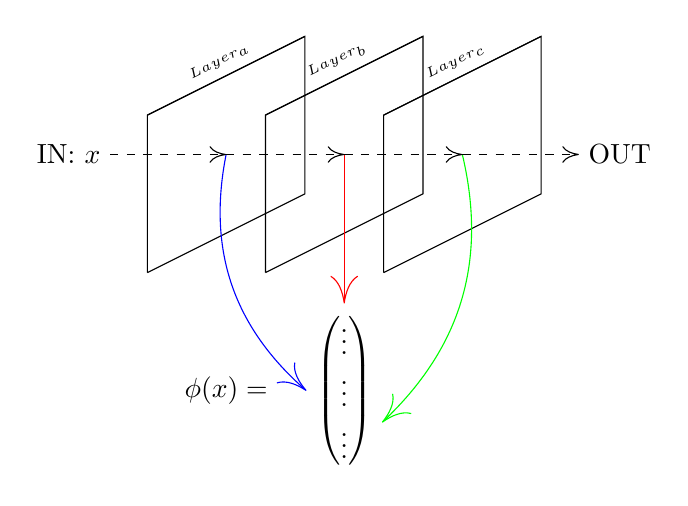
\begin{tikzpicture}[-]

\coordinate (00) at (0,0) {};
\coordinate (01) at (2,1) {};
\coordinate (02) at (2,3) {};
\coordinate (03) at (0,2) {};
\coordinate (0M) at (1,1.5) {};

\coordinate (10) at (1.5,0) {};
\coordinate (11) at (3.5,1) {};
\coordinate (12) at (3.5,3) {};
\coordinate (13) at (1.5,2) {};
\coordinate (1M) at (2.5,1.5) {};

\coordinate (20) at (3,0) {};
\coordinate (21) at (5,1) {};
\coordinate (22) at (5,3) {};
\coordinate (23) at (3,2) {}; 
\coordinate (2M) at (4,1.5) {};

\node (vector) at (2.5,-1.5) {$\begin{pmatrix}
		\vdots \\
 		\vdots \\
 		\vdots
 		
	\end{pmatrix}$};
\node (in) at (-1,1.5) {IN: $x$};
\node (out) at (6,1.5) {OUT};
\node (phi) at (1,-1.5) {$\phi(x)=$};

\draw (00) -- (01) -- (02) -- (03) -- (00);
\draw (10) -- (11) -- (12) -- (13) -- (10);
\draw (20) -- (21) -- (22) -- (23) -- (20);

\draw (02) -- (03) node [above, sloped, pos=0.5] {\tiny $Layer_a$};
\draw (12) -- (13) node [above, sloped, pos=0.5] {\tiny $Layer_b$};
\draw (22) -- (23) node [above, sloped, pos=0.5] {\tiny $Layer_c$};

\draw[blue,-{>[scale=5,length=2,width=2]}] (0M) to [bend right] (vector.west);
\draw[red,-{>[scale=5,length=2,width=2]}] (1M) to (vector.north);
\draw[green,-{>[scale=5,length=2,width=2]}] (2M) to [bend left] (vector.320);
\draw[-{>[scale=3,length=2,width=2]},dashed] (in) to (0M);
\draw[-{>[scale=3,length=2,width=2]},dashed] (0M) to (1M);
\draw[-{>[scale=3,length=2,width=2]},dashed] (1M) to (2M);
\draw[-{>[scale=3,length=2,width=2]},dashed] (2M) to (out);


\end{tikzpicture}	
		\end{center}
	\end{itemize}
\end{frame}

\begin{frame}{Basic Idea}
	\begin{itemize}
		\item Take $k$ nearest neighbor images with existing attribute: $S^+$
		\item Take $k$ nearest neighbor images with missing attribute: $S^-$
		\vfill
		\pause
		
		\item $\phi^+ = \phi(S^+)$ and $\phi^- = \phi(S^-)$
		\item Build the mean $\overline{\phi^+}$ and $\overline{\phi^-}$
		\vfill
		\pause 
		
		\item Representation of attribute: $w=\overline{\phi^+}-\overline{\phi^-}$
	\end{itemize}
\end{frame}

\begin{frame}{Basic Idea}
	How to get the output picture?
	
	\vfill
	\pause
	
	\begin{itemize}
		\item $\phi(z) = \phi(x) + \alpha w$
		\item Reverse mapping of $\phi(z)$ into pixel space:
		
		\vfill
		\pause
		\begin{itemize}
			\item $\tilde{z} = \underset{\tilde{z}}{\mathrm{argmin}} \frac{1}{2} ||\phi(z)-\phi(\tilde{z})||_2^2 + \lambda R_{\beta}(\tilde{z})$ 
			\item with $R_{\beta}(\tilde{z}) = \sum_{i,j}((\tilde{z}_{i,j+1}-\tilde{z}_{i,j})^2 + (\tilde{z}_{i+1,j}-\tilde{z}_{i,j})^2)^{\frac{\beta}{2}}$
		\end{itemize}
		 
	\end{itemize}
	
\end{frame}

\begin{frame}{Technical}
	\begin{itemize}
		\item Model: VGG19 pretrained on IMAGENET dataset
		\item $\phi(x)$: third, fourth and fifth Relu Layer
		\item Regularization parameters: $\beta=2$, $\lambda = 0.001$
		\item Test set: labeled faces in the wild (LFW dataset)
		\item Optimizer: Adam
		\item KNN: on discrete attribute features (mustache, smiling, $\dots$)
		\item Normalization: $\phi(x) = \frac{\phi(x)}{||\phi(x)||}$, $w = \frac{w}{||w||}$
	\end{itemize} 
\end{frame}


% eyeglasses

\begin{frame}{Results: Eyeglasses}{$\alpha=0.4$, $k=100$}
	\centering
	\begin{minipage}{81px}
		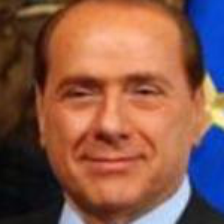
\includegraphics[width=80px]{../pictures/outputs/start-imgs/Berlusconi.png}\\
		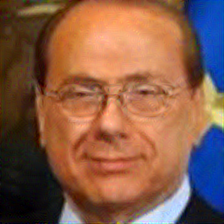
\includegraphics[width=80px]{../pictures/outputs/eyeglasses_alpha0.4_k100/Berlusconi.png}
	\end{minipage}%
	\begin{minipage}{81px}
		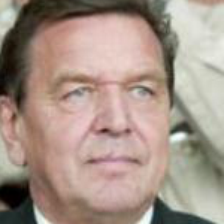
\includegraphics[width=80px]{../pictures/outputs/start-imgs/Schroeder.png}\\
		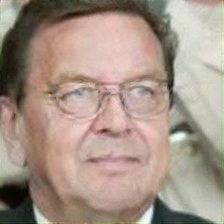
\includegraphics[width=80px]{../pictures/outputs/eyeglasses_alpha0.4_k100/Schroeder.png}
	\end{minipage}%
	\begin{minipage}{81px}
		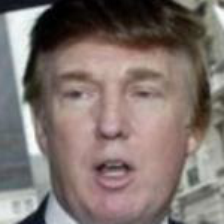
\includegraphics[width=80px]{../pictures/outputs/start-imgs/Trump.png}\\
		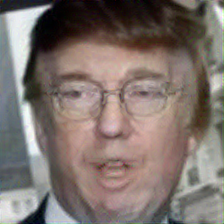
\includegraphics[width=80px]{../pictures/outputs/eyeglasses_alpha0.4_k100/Trump.png}
	\end{minipage}%
	\begin{minipage}{81px}
		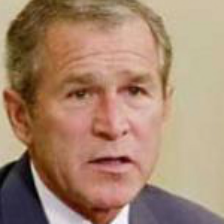
\includegraphics[width=80px]{../pictures/outputs/start-imgs/Bush.png}\\
		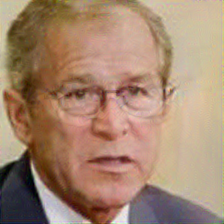
\includegraphics[width=80px]{../pictures/outputs/eyeglasses_alpha0.4_k100/Bush.png}
	\end{minipage}
\end{frame}

% sunglasses

\begin{frame}{Results: Sunglasses}{$\alpha=0.4$, $k=100$}
	\centering
	\begin{minipage}{81px}
		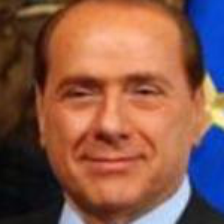
\includegraphics[width=80px]{../pictures/outputs/start-imgs/Berlusconi.png}\\
		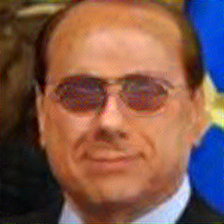
\includegraphics[width=80px]{../pictures/outputs/sunglasses_alpha0.4_k100/Berlusconi.png}
	\end{minipage}%
	\begin{minipage}{81px}
		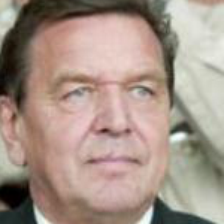
\includegraphics[width=80px]{../pictures/outputs/start-imgs/Schroeder.png}\\
		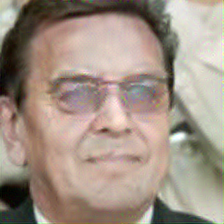
\includegraphics[width=80px]{../pictures/outputs/sunglasses_alpha0.4_k100/Schroeder.png}
	\end{minipage}%
	\begin{minipage}{81px}
		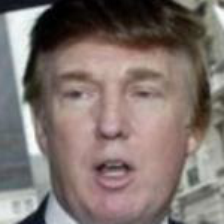
\includegraphics[width=80px]{../pictures/outputs/start-imgs/Trump.png}\\
		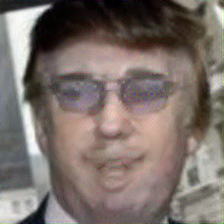
\includegraphics[width=80px]{../pictures/outputs/sunglasses_alpha0.4_k100/Trump.png}
	\end{minipage}%
	\begin{minipage}{81px}
		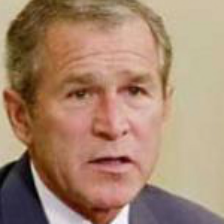
\includegraphics[width=80px]{../pictures/outputs/start-imgs/Bush.png}\\
		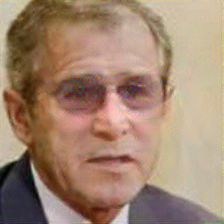
\includegraphics[width=80px]{../pictures/outputs/sunglasses_alpha0.4_k100/Bush.png}
	\end{minipage}
\end{frame}

% mouth_open

\begin{frame}{Results: Mouth open}{$\alpha=0.4$, $k=100$}
	\centering
	\begin{minipage}{81px}
		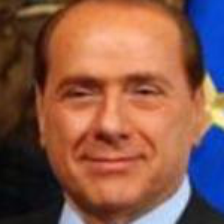
\includegraphics[width=80px]{../pictures/outputs/start-imgs/Berlusconi.png}\\
		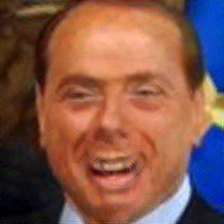
\includegraphics[width=80px]{../pictures/outputs/mouth_open_alpha0.4_k100/Berlusconi.png}
	\end{minipage}%
	\begin{minipage}{81px}
		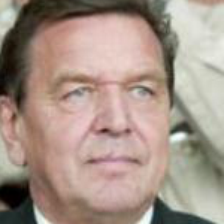
\includegraphics[width=80px]{../pictures/outputs/start-imgs/Schroeder.png}\\
		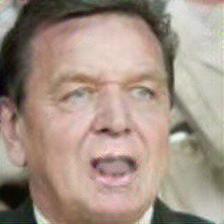
\includegraphics[width=80px]{../pictures/outputs/mouth_open_alpha0.4_k100/Schroeder.png}
	\end{minipage}%
	\begin{minipage}{81px}
		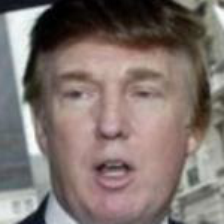
\includegraphics[width=80px]{../pictures/outputs/start-imgs/Trump.png}\\
		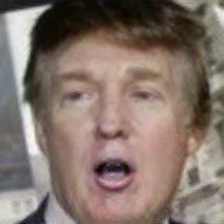
\includegraphics[width=80px]{../pictures/outputs/mouth_open_alpha0.4_k100/Trump.png}
	\end{minipage}%
	\begin{minipage}{81px}
		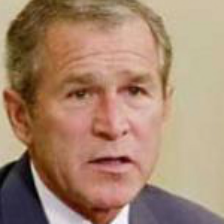
\includegraphics[width=80px]{../pictures/outputs/start-imgs/Bush.png}\\
		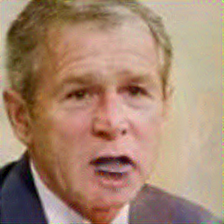
\includegraphics[width=80px]{../pictures/outputs/mouth_open_alpha0.4_k100/Bush.png}
	\end{minipage}
\end{frame}

% female

\begin{frame}{Results: Female}{$\alpha=0.4$, $k=100$}
	\centering
	\begin{minipage}{81px}
		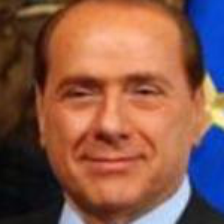
\includegraphics[width=80px]{../pictures/outputs/start-imgs/Berlusconi.png}\\
		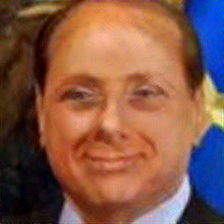
\includegraphics[width=80px]{../pictures/outputs/female_alpha0.4_k100/Berlusconi.png}
	\end{minipage}%
	\begin{minipage}{81px}
		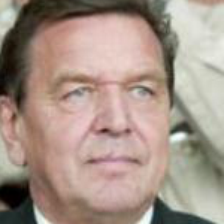
\includegraphics[width=80px]{../pictures/outputs/start-imgs/Schroeder.png}\\
		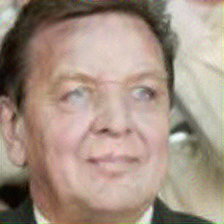
\includegraphics[width=80px]{../pictures/outputs/female_alpha0.4_k100/Schroeder.png}
	\end{minipage}%
	\begin{minipage}{81px}
		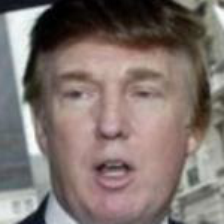
\includegraphics[width=80px]{../pictures/outputs/start-imgs/Trump.png}\\
		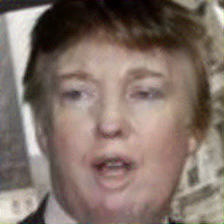
\includegraphics[width=80px]{../pictures/outputs/female_alpha0.4_k100/Trump.png}
	\end{minipage}%
	\begin{minipage}{81px}
		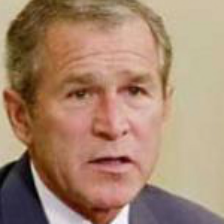
\includegraphics[width=80px]{../pictures/outputs/start-imgs/Bush.png}\\
		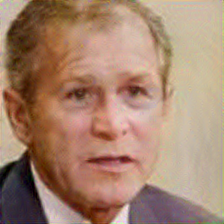
\includegraphics[width=80px]{../pictures/outputs/female_alpha0.4_k100/Bush.png}
	\end{minipage}
\end{frame}

% heavy_makeup

\begin{frame}{Results: Heavy makeup}{$\alpha=0.4$, $k=100$}
	\centering
	\begin{minipage}{81px}
		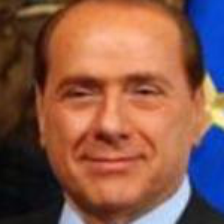
\includegraphics[width=80px]{../pictures/outputs/start-imgs/Berlusconi.png}\\
		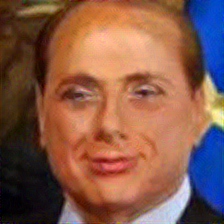
\includegraphics[width=80px]{../pictures/outputs/heavy_makeup_alpha0.4_k100/Berlusconi.png}
	\end{minipage}%
	\begin{minipage}{81px}
		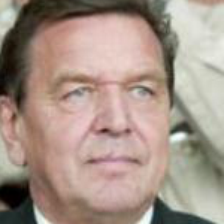
\includegraphics[width=80px]{../pictures/outputs/start-imgs/Schroeder.png}\\
		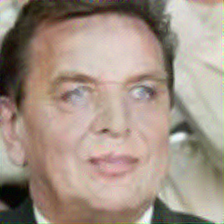
\includegraphics[width=80px]{../pictures/outputs/heavy_makeup_alpha0.4_k100/Schroeder.png}
	\end{minipage}%
	\begin{minipage}{81px}
		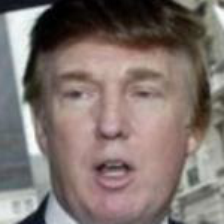
\includegraphics[width=80px]{../pictures/outputs/start-imgs/Trump.png}\\
		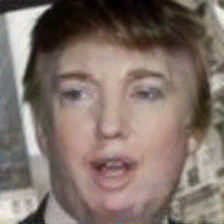
\includegraphics[width=80px]{../pictures/outputs/heavy_makeup_alpha0.4_k100/Trump.png}
	\end{minipage}%
	\begin{minipage}{81px}
		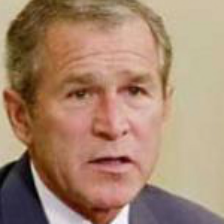
\includegraphics[width=80px]{../pictures/outputs/start-imgs/Bush.png}\\
		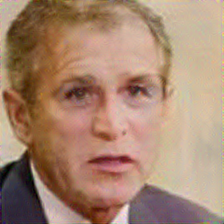
\includegraphics[width=80px]{../pictures/outputs/heavy_makeup_alpha0.4_k100/Bush.png}
	\end{minipage}
\end{frame}

% smiling

\begin{frame}{Results: Smiling}{$\alpha=0.4$, $k=100$}
	\centering
	\begin{minipage}{81px}
		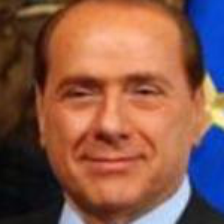
\includegraphics[width=80px]{../pictures/outputs/start-imgs/Berlusconi.png}\\
		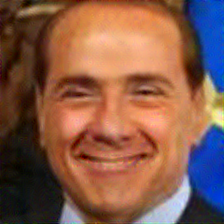
\includegraphics[width=80px]{../pictures/outputs/smiling_alpha0.4_k100/Berlusconi.png}
	\end{minipage}%
	\begin{minipage}{81px}
		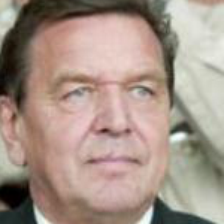
\includegraphics[width=80px]{../pictures/outputs/start-imgs/Schroeder.png}\\
		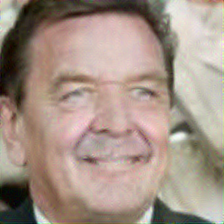
\includegraphics[width=80px]{../pictures/outputs/smiling_alpha0.4_k100/Schroeder.png}
	\end{minipage}%
	\begin{minipage}{81px}
		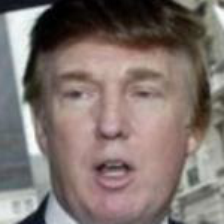
\includegraphics[width=80px]{../pictures/outputs/start-imgs/Trump.png}\\
		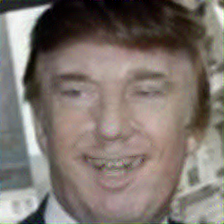
\includegraphics[width=80px]{../pictures/outputs/smiling_alpha0.4_k100/Trump.png}
	\end{minipage}%
	\begin{minipage}{81px}
		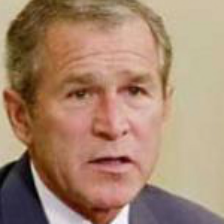
\includegraphics[width=80px]{../pictures/outputs/start-imgs/Bush.png}\\
		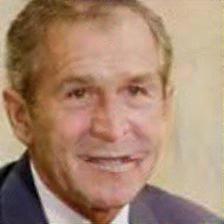
\includegraphics[width=80px]{../pictures/outputs/smiling_alpha0.4_k100/Bush.png}
	\end{minipage}
\end{frame}

% mustache

\begin{frame}{Results: Mustache}{$\alpha=0.4$, $k=100$}
	\centering
	\begin{minipage}{81px}
		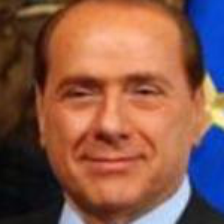
\includegraphics[width=80px]{../pictures/outputs/start-imgs/Berlusconi.png}\\
		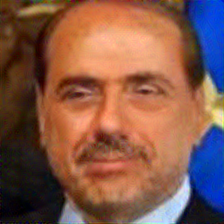
\includegraphics[width=80px]{../pictures/outputs/mustache_alpha0.4_k100/Berlusconi.png}
	\end{minipage}%
	\begin{minipage}{81px}
		\includegraphics[width=80px]{../pictures/outputs/start-imgs/Schroeder.png}\\
		\includegraphics[width=80px]{../pictures/outputs/mustache_alpha0.4_k100/Schroeder.png}
	\end{minipage}%
	\begin{minipage}{81px}
		\includegraphics[width=80px]{../pictures/outputs/start-imgs/Trump.png}\\
		\includegraphics[width=80px]{../pictures/outputs/mustache_alpha0.4_k100/Trump.png}
	\end{minipage}%
	\begin{minipage}{81px}
		\includegraphics[width=80px]{../pictures/outputs/start-imgs/Bush.png}\\
		\includegraphics[width=80px]{../pictures/outputs/mustache_alpha0.4_k100/Bush.png}
	\end{minipage}
\end{frame}

% asian

\begin{frame}{Results: Asian}{$\alpha=0.4$, $k=100$}
	\centering
	\begin{minipage}{81px}
		\includegraphics[width=80px]{../pictures/outputs/start-imgs/Berlusconi.png}\\
		\includegraphics[width=80px]{../pictures/outputs/asian_alpha0.4_k100/Berlusconi.png}
	\end{minipage}%
	\begin{minipage}{81px}
		\includegraphics[width=80px]{../pictures/outputs/start-imgs/Schroeder.png}\\
		\includegraphics[width=80px]{../pictures/outputs/asian_alpha0.4_k100/Schroeder.png}
	\end{minipage}%
	\begin{minipage}{81px}
		\includegraphics[width=80px]{../pictures/outputs/start-imgs/Trump.png}\\
		\includegraphics[width=80px]{../pictures/outputs/asian_alpha0.4_k100/Trump.png}
	\end{minipage}%
	\begin{minipage}{81px}
		\includegraphics[width=80px]{../pictures/outputs/start-imgs/Bush.png}\\
		\includegraphics[width=80px]{../pictures/outputs/asian_alpha0.4_k100/Bush.png}
	\end{minipage}
\end{frame}

\begin{frame}{Varying the parameters: Senior}{$k=100$, $\alpha \in [0.3, 0.4, \dots, 1.0]$}
	\centering
	\begin{minipage}{81px}
		\includegraphics[width=80px]{../pictures/outputs/alpha_k/Senior/k100/Silvio_Berlusconi_0023_alpha-0.3_k-1002017-02-07_13-39-13.png}\\
		\includegraphics[width=80px]{../pictures/outputs/alpha_k/Senior/k100/Silvio_Berlusconi_0023_alpha-0.7_k-1002017-02-07_15-39-04.png}
	\end{minipage}%
	\begin{minipage}{81px}
		\includegraphics[width=80px]{../pictures/outputs/alpha_k/Senior/k100/Silvio_Berlusconi_0023_alpha-0.4_k-1002017-02-07_14-02-37.png}\\
		\includegraphics[width=80px]{../pictures/outputs/alpha_k/Senior/k100/Silvio_Berlusconi_0023_alpha-0.8_k-1002017-02-07_16-16-14.png}
	\end{minipage}%
	\begin{minipage}{81px}
		\includegraphics[width=80px]{../pictures/outputs/alpha_k/Senior/k100/Silvio_Berlusconi_0023_alpha-0.5_k-1002017-02-07_14-28-35.png}\\
		\includegraphics[width=80px]{../pictures/outputs/alpha_k/Senior/k100/Silvio_Berlusconi_0023_alpha-0.9_k-1002017-02-07_16-42-01.png}
	\end{minipage}%
	\begin{minipage}{81px}
		\includegraphics[width=80px]{../pictures/outputs/alpha_k/Senior/k100/Silvio_Berlusconi_0023_alpha-0.6_k-1002017-02-07_15-00-08.png}\\
		\includegraphics[width=80px]{../pictures/outputs/alpha_k/Senior/k100/Silvio_Berlusconi_0023_alpha-1.0_k-1002017-02-07_17-07-47.png}
	\end{minipage}
\end{frame}

\begin{frame}{Varying the parameters: Senior}{$k \in [1, 10, 20, 50, 75, 100, 150, 200]$, $\alpha=0.5$}
	\centering
	\begin{minipage}{81px}
		\includegraphics[width=80px]{../pictures/outputs/alpha_k/Senior/alpha0.5/Silvio_Berlusconi_0023_alpha-0.5_k-12017-02-07_14-20-42.png}\\
		\includegraphics[width=80px]{../pictures/outputs/alpha_k/Senior/alpha0.5/Silvio_Berlusconi_0023_alpha-0.5_k-752017-02-07_14-26-56.png}
	\end{minipage}%
	\begin{minipage}{81px}
		\includegraphics[width=80px]{../pictures/outputs/alpha_k/Senior/alpha0.5/Silvio_Berlusconi_0023_alpha-0.5_k-102017-02-07_14-22-13.png}\\
		\includegraphics[width=80px]{../pictures/outputs/alpha_k/Senior/alpha0.5/Silvio_Berlusconi_0023_alpha-0.5_k-1002017-02-07_14-28-35.png}
	\end{minipage}%
	\begin{minipage}{81px}
		\includegraphics[width=80px]{../pictures/outputs/alpha_k/Senior/alpha0.5/Silvio_Berlusconi_0023_alpha-0.5_k-202017-02-07_14-23-45.png}\\
		\includegraphics[width=80px]{../pictures/outputs/alpha_k/Senior/alpha0.5/Silvio_Berlusconi_0023_alpha-0.5_k-1502017-02-07_14-30-17.png}
	\end{minipage}%
	\begin{minipage}{81px}
		\includegraphics[width=80px]{../pictures/outputs/alpha_k/Senior/alpha0.5/Silvio_Berlusconi_0023_alpha-0.5_k-502017-02-07_14-25-20.png}\\
		\includegraphics[width=80px]{../pictures/outputs/alpha_k/Senior/alpha0.5/Silvio_Berlusconi_0023_alpha-0.5_k-2002017-02-07_14-32-10.png}
	\end{minipage}%
\end{frame}


\begin{frame}{Varying the parameters: Smiling}{$k=100$, $\alpha \in [0.3, 0.4, \dots, 1.0]$}
	\centering
	\begin{minipage}{81px}
		\includegraphics[width=80px]{../pictures/outputs/alpha_k/Smiling/k100/Silvio_Berlusconi_0023_alpha-0.3_k-1002017-02-07_13-52-13.png}\\
		\includegraphics[width=80px]{../pictures/outputs/alpha_k/Smiling/k100/Silvio_Berlusconi_0023_alpha-0.7_k-1002017-02-07_15-58-35.png}
	\end{minipage}%
	\begin{minipage}{81px}
		\includegraphics[width=80px]{../pictures/outputs/alpha_k/Smiling/k100/Silvio_Berlusconi_0023_alpha-0.4_k-1002017-02-07_14-15-38.png}\\
		\includegraphics[width=80px]{../pictures/outputs/alpha_k/Smiling/k100/Silvio_Berlusconi_0023_alpha-0.8_k-1002017-02-07_16-29-08.png}
	\end{minipage}%
	\begin{minipage}{81px}
		\includegraphics[width=80px]{../pictures/outputs/alpha_k/Smiling/k100/Silvio_Berlusconi_0023_alpha-0.5_k-1002017-02-07_14-41-42.png}\\
		\includegraphics[width=80px]{../pictures/outputs/alpha_k/Smiling/k100/Silvio_Berlusconi_0023_alpha-0.9_k-1002017-02-07_16-54-53.png}
	\end{minipage}%
	\begin{minipage}{81px}
		\includegraphics[width=80px]{../pictures/outputs/alpha_k/Smiling/k100/Silvio_Berlusconi_0023_alpha-0.6_k-1002017-02-07_15-19-24.png}\\
		\includegraphics[width=80px]{../pictures/outputs/alpha_k/Smiling/k100/Silvio_Berlusconi_0023_alpha-1.0_k-1002017-02-07_17-20-40.png}
	\end{minipage}
\end{frame}

\begin{frame}{Varying the parameters: Smiling}{$k \in [1, 10, 20, 50, 75, 100, 150, 200]$, $\alpha=0.5$}
	\centering
	\begin{minipage}{81px}
		\includegraphics[width=80px]{../pictures/outputs/alpha_k/Smiling/alpha0.4/Silvio_Berlusconi_0023_alpha-0.4_k-12017-02-07_14-07-41.png}\\
		\includegraphics[width=80px]{../pictures/outputs/alpha_k/Smiling/alpha0.4/Silvio_Berlusconi_0023_alpha-0.4_k-752017-02-07_14-13-59.png}
	\end{minipage}%
	\begin{minipage}{81px}
		\includegraphics[width=80px]{../pictures/outputs/alpha_k/Smiling/alpha0.4/Silvio_Berlusconi_0023_alpha-0.4_k-102017-02-07_14-09-14.png}\\
		\includegraphics[width=80px]{../pictures/outputs/alpha_k/Smiling/alpha0.4/Silvio_Berlusconi_0023_alpha-0.4_k-1002017-02-07_14-15-38.png}
	\end{minipage}%
	\begin{minipage}{81px}
		\includegraphics[width=80px]{../pictures/outputs/alpha_k/Smiling/alpha0.4/Silvio_Berlusconi_0023_alpha-0.4_k-202017-02-07_14-10-46.png}\\
		\includegraphics[width=80px]{../pictures/outputs/alpha_k/Smiling/alpha0.4/Silvio_Berlusconi_0023_alpha-0.4_k-1502017-02-07_14-17-20.png}
	\end{minipage}%
	\begin{minipage}{81px}
		\includegraphics[width=80px]{../pictures/outputs/alpha_k/Smiling/alpha0.4/Silvio_Berlusconi_0023_alpha-0.4_k-502017-02-07_14-12-22.png}\\
		\includegraphics[width=80px]{../pictures/outputs/alpha_k/Smiling/alpha0.4/Silvio_Berlusconi_0023_alpha-0.4_k-2002017-02-07_14-19-11.png}
	\end{minipage}%
\end{frame}


\begin{frame}{Outlook}
	\begin{itemize}
		\item Multiple features at once: $\phi(z) = \phi(x) + \alpha \sum_{i} w_i$
		\item Nearest Neighbor in deep feature space
		\item Choose more/less/other layers for $\phi$
		\item Change normalization: $w = w\frac{||\phi(x)||}{||w||}$
	\end{itemize}
\end{frame}

\end{document}
